\documentclass[border=10pt]{standalone}

\usepackage{tikz}
\usepackage{tikzsymbols}
\usetikzlibrary{calc,patterns,shapes.geometric}

\def\centerarc[#1](#2)(#3:#4:#5){\draw[#1] ($(#2)+({#5*cos(#3)},{#5*sin(#3)})$) arc (#3:#4:#5);}

\begin{document}
	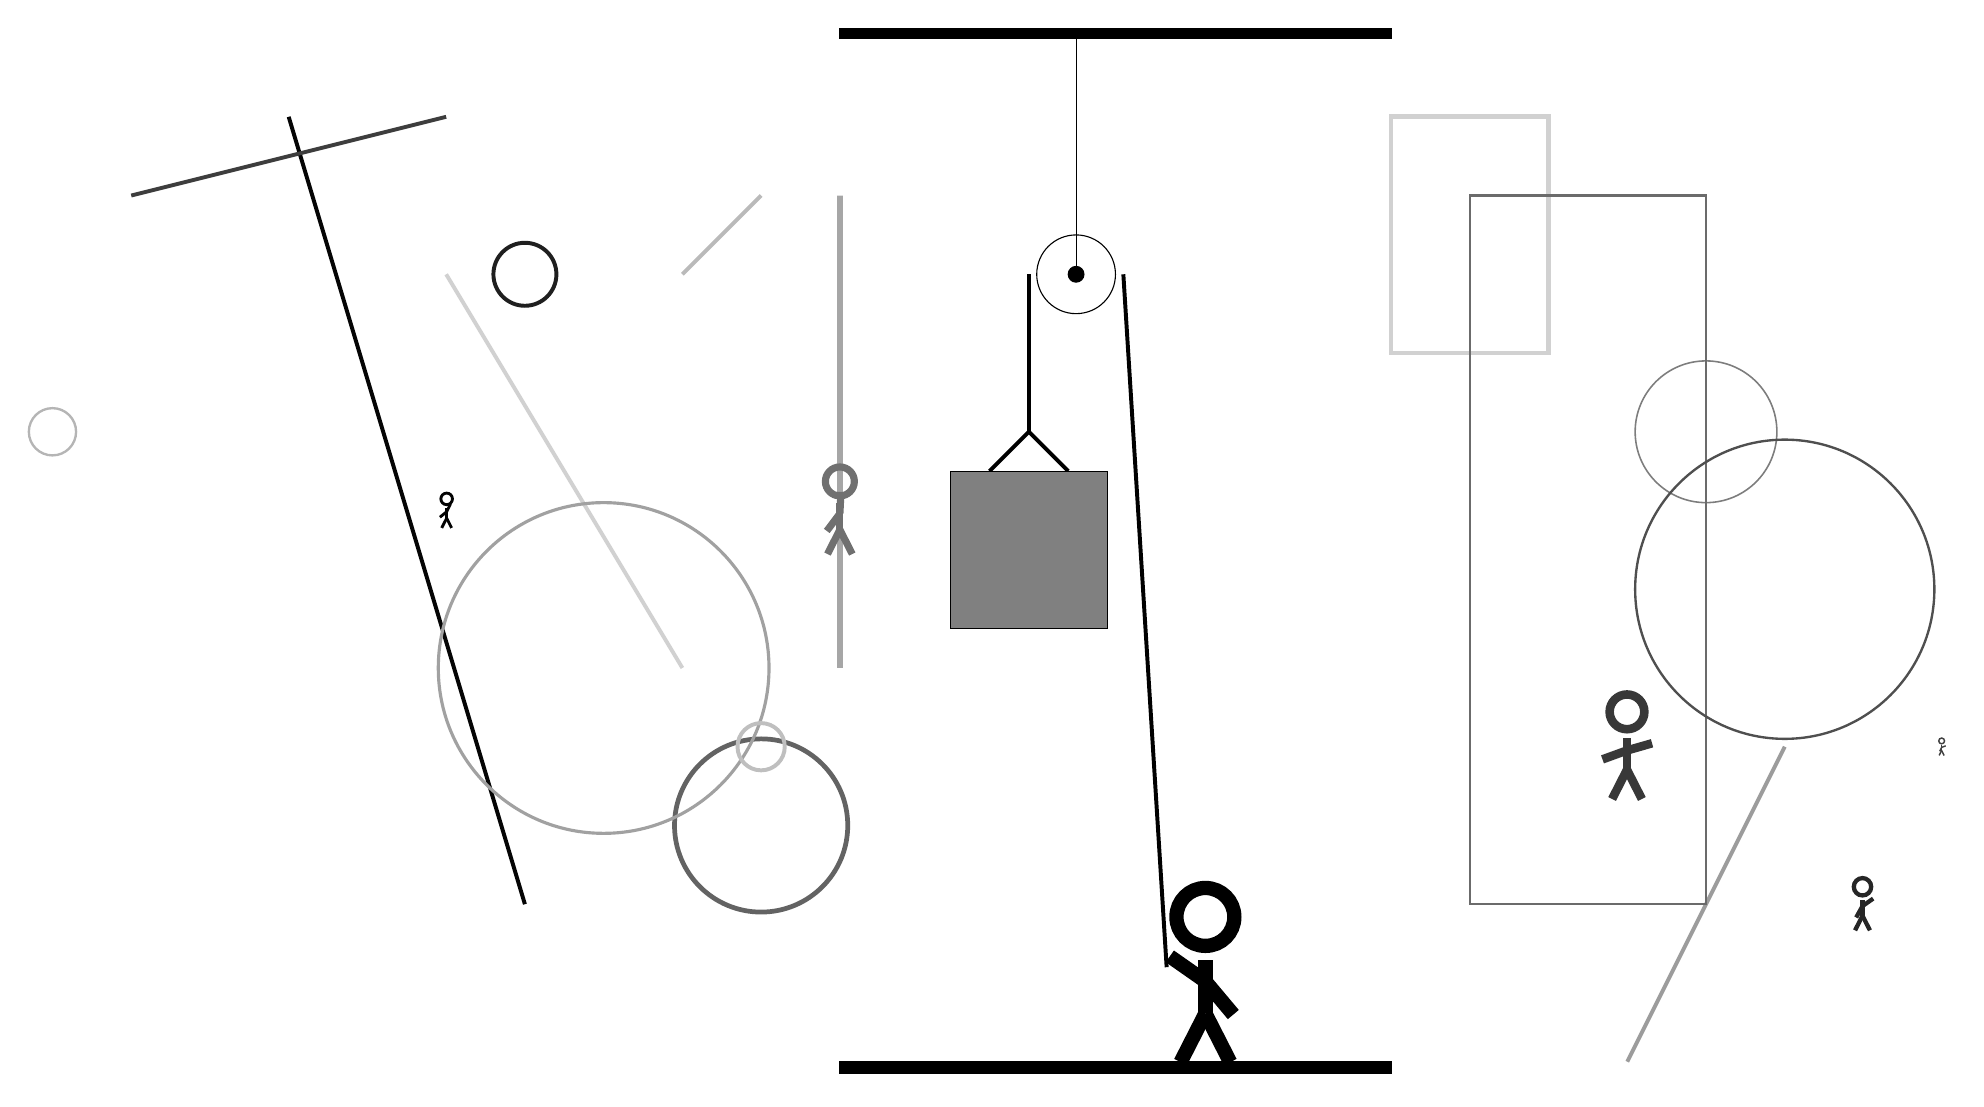
\begin{tikzpicture}
		%%%%% START %%%%%
		
		\draw[fill=black] (-2, 10) rectangle (5, 10.125);
		
		\draw (1, 7) circle (0.5);
		\draw[fill=black] (1, 7) circle (0.1);
		\draw (1, 10) -- (1, 7);
		
		\draw[line width=0.5mm] (-0.1, 4.5) -- (0.4, 5.0) -- (0.9, 4.5);
		\draw[fill=black!50] (-0.6, 4.5) rectangle (1.4, 2.5);
		
		\draw[line width=0.5mm, color=black!39](10, 1) -- (8, -3);
		
		\draw[line width=0.5mm, color=black!98](-6, -1) -- (-9, 9);
		\node[line width=0.7mm, color=black!78] at (8, 1) {\Strichmaxerl[6][20][16]};
		\draw[line width=0.7mm, color=black!35] (-2, 8) rectangle (-2, 2);
		
		\draw[line width=0.5mm, color=black!27](-4, 7) -- (-3, 8);
		
		\draw [line width=0.5mm, color=black!88](-6, 7) circle (0.4);
		
		\draw[line width=0.6mm, color=black!18] (5, 9) rectangle (7, 6);
		
		\node[line width=0.6mm, color=black!85] at (11, -1) {\Strichmaxerl[3][61][35]};
		\draw [line width=0.3mm, color=black!29](-12, 5) circle (0.3);
		\draw [line width=0.2mm, color=black!51](9, 5) circle (0.9);
		\draw [line width=0.6mm, color=black!61](-3, 0) circle (1.1);
		\draw[line width=0.3mm, color=black!58] (6, 8) rectangle (9, -1);
		\draw[line width=0.5mm, color=black!76](-7, 9) -- (-11, 8);
		\draw[line width=0.5mm, color=black!18](-7, 7) -- (-4, 2);
		\draw[line width=0.5mm, color=black!63] (-4, 9) rectangle (-4, 9);
		\draw [line width=0.4mm, color=black!37](-5, 2) circle (2.1);
		
		\node[line width=0.4mm, color=black!99] at (-7, 4) {\Strichmaxerl[2][39][64]};
		\draw [line width=0.5mm, color=black!25](-3, 1) circle (0.3);
		\node[line width=0.3mm, color=black!56] at (-2, 4) {\Strichmaxerl[5][53][87]};
		
		\node[line width=0.2mm, color=black!75] at (12, 1) {\Strichmaxerl[1][64][20]};
		\draw [line width=0.3mm, color=black!69](10, 3) circle (1.9);
		
		
		\draw[line width=0.5mm] (0.4, 7) -- (0.4, 5.0);
		\centerarc[line width=0.5mm](1, 7)(0:180:0.6);
		\draw[line width=0.5mm](1.6, 7) -- (2.15, -1.8);
		
		\node at (2.6, -1.9) {\Strichmaxerl[10][-35][-50]};
		
		\draw[fill=black] (-2, -3) rectangle (5, -3.15);
		
		%%%%% END %%%%%
	\end{tikzpicture}
\end{document}